 \providecommand{\main}{../../..}
\documentclass[\main/main.tex]{subfiles}
\begin{document}
\subsection{Esercizio 1}
Dato il seguente problema di PL, si risolva graficamente e si ottenga il valore della soluzione ottima e di tutte le variabili di scarto.

Si ricavi, per via grafica, per quali valori di $c_2$, inizialmente pari a $-1$, la \textbf{composizione} della base ottima non cambia.

\begin{figure}
  \begin{align*}
    \max z = 2x_1 - x_2         \\
    x_1 + 2x_2 & \leq 4         \\
    2x_1 + x_2 & \geq 2         \\
    x_1 - 2x_2 & \leq 6         \\
    x_1        & \geq 0         \\
    x_2        & \in \mathbb{R}
  \end{align*}
  \caption{Esercizio 1}
\end{figure}

\subsection{Soluzione esercizio 1}

\subsubsection*{Disegno l'area di definizione del problema}
\begin{figure}
  \begin{subfigure}{0.45\textwidth}
    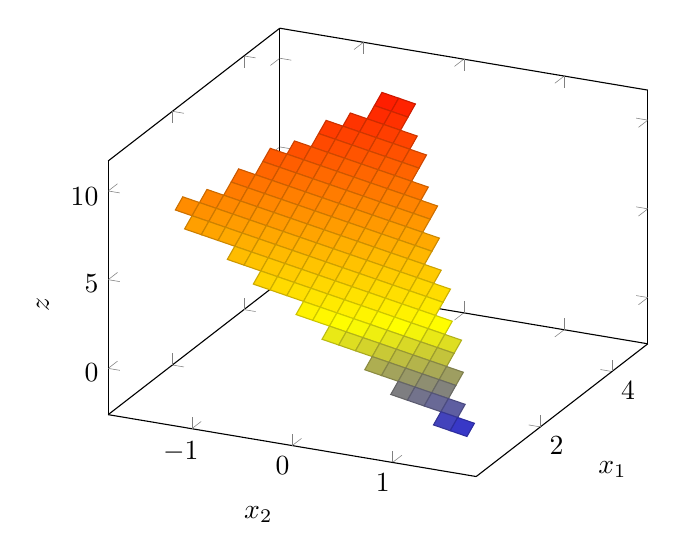
\begin{tikzpicture}
      \begin{axis}[
          xlabel=$x_2$,
          ylabel=$x_1$,
          zlabel=$z$,
          domain=-2:2,
          y domain=0:5
        ]
        \addplot3[surf, unbounded coords=jump]
        {
          y+2*x<=4 &&
          2*y +x >= 2 &&
          y -2*x <= 6 ?
          2*y-x:NaN
        };
      \end{axis}
    \end{tikzpicture}
    \caption{La funzione $z$}
  \end{subfigure}
  \begin{subfigure}{0.45\textwidth}
    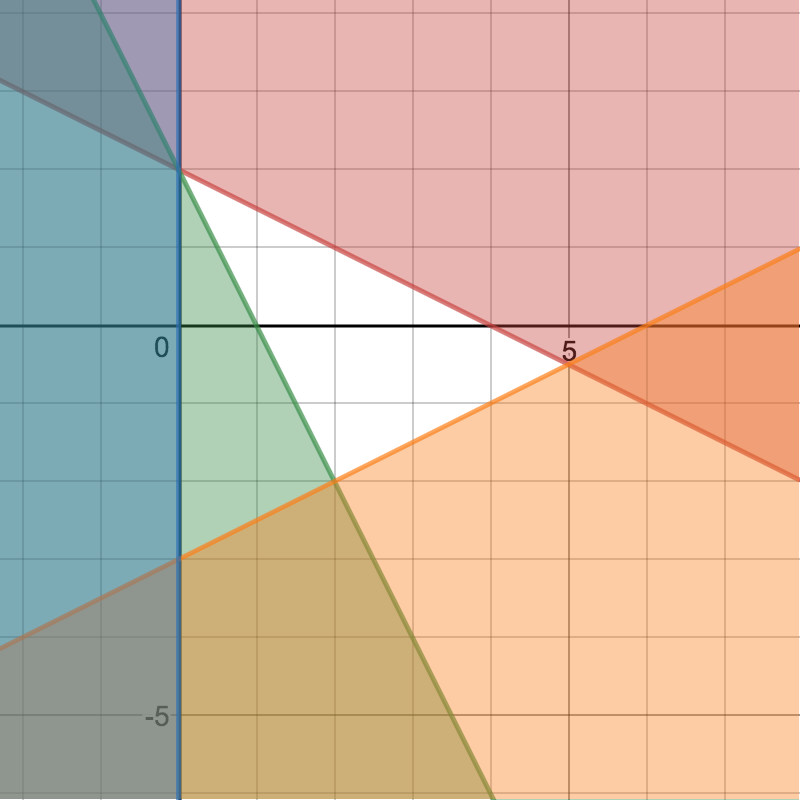
\includegraphics[width=0.8\textwidth]{2016_11_16}
    \caption{Regione di definizione del problema}
  \end{subfigure}
\end{figure}

\subsubsection*{Identifico il punto di massimo}
Il punto di massimo si trova all'intersezione tra primo e terzo vincolo:
\[
  \begin{cases}
    x_1 + 2x_2 = 4 \\
    x_1 - 2x_2 = 6
  \end{cases}
  \Rightarrow
  \begin{cases}
    x_2 = -\frac{1}{2} \\
    x_1 = 5
  \end{cases}
\]

\begin{align*}
  x_1 & = 5             \\
  x_2 & = -\frac{1}{2}  \\
  s_1 & = 0             \\
  s_2 & = -\frac{15}{2} \\
  s_3 & = 0
\end{align*}

\subsubsection*{Analisi di sensitività}

\begin{figure}
  \begin{subfigure}{0.45\textwidth}
    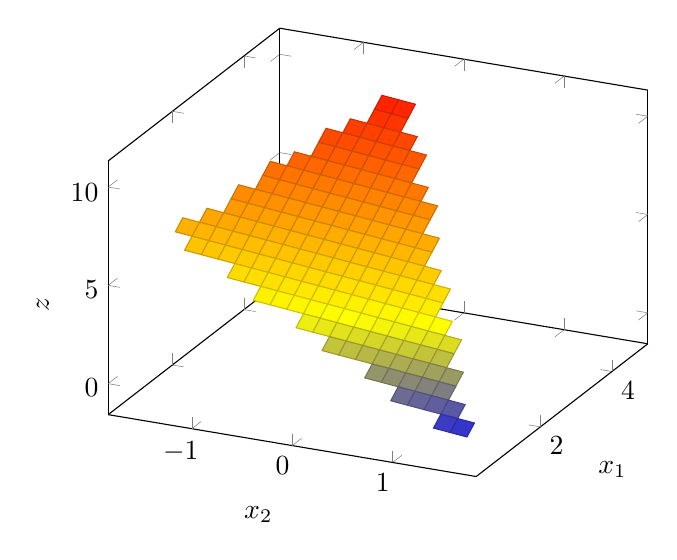
\begin{tikzpicture}
      \begin{axis}[
          xlabel=$x_2$,
          ylabel=$x_1$,
          zlabel=$z$,
          domain=-2:2,
          y domain=0:5
        ]
        \addplot3[surf, unbounded coords=jump]
        {
          y+2*x<=4 &&
          2*y +x >= 2 &&
          y -2*x <= 6 ?
          2*y+(-1+0.5)*x:NaN
        };
      \end{axis}
    \end{tikzpicture}
    \caption{La funzione $z$}
  \end{subfigure}
  \begin{subfigure}{0.45\textwidth}
    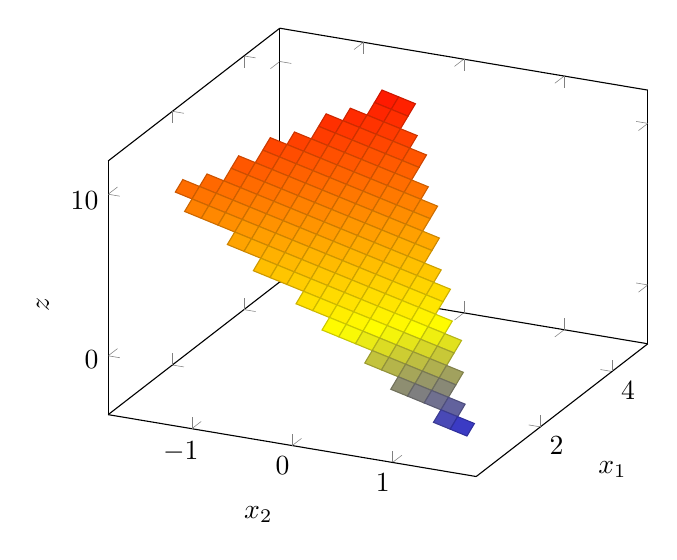
\begin{tikzpicture}
      \begin{axis}[
          xlabel=$x_2$,
          ylabel=$x_1$,
          zlabel=$z$,
          domain=-2:2,
          y domain=0:5
        ]
        \addplot3[surf, unbounded coords=jump]
        {
          y+2*x<=4 &&
          2*y +x >= 2 &&
          y -2*x <= 6 ?
          2*y+(-1-0.5)*x:NaN
        };
      \end{axis}
    \end{tikzpicture}
    \caption{La funzione $z$}
  \end{subfigure}
\end{figure}

\end{document}